\section{Tokenformer}
\label{sec:tokenformer}
\begin{frame}
\frametitle{TokenFormer}
\begin{figure}[h]
    \centering
    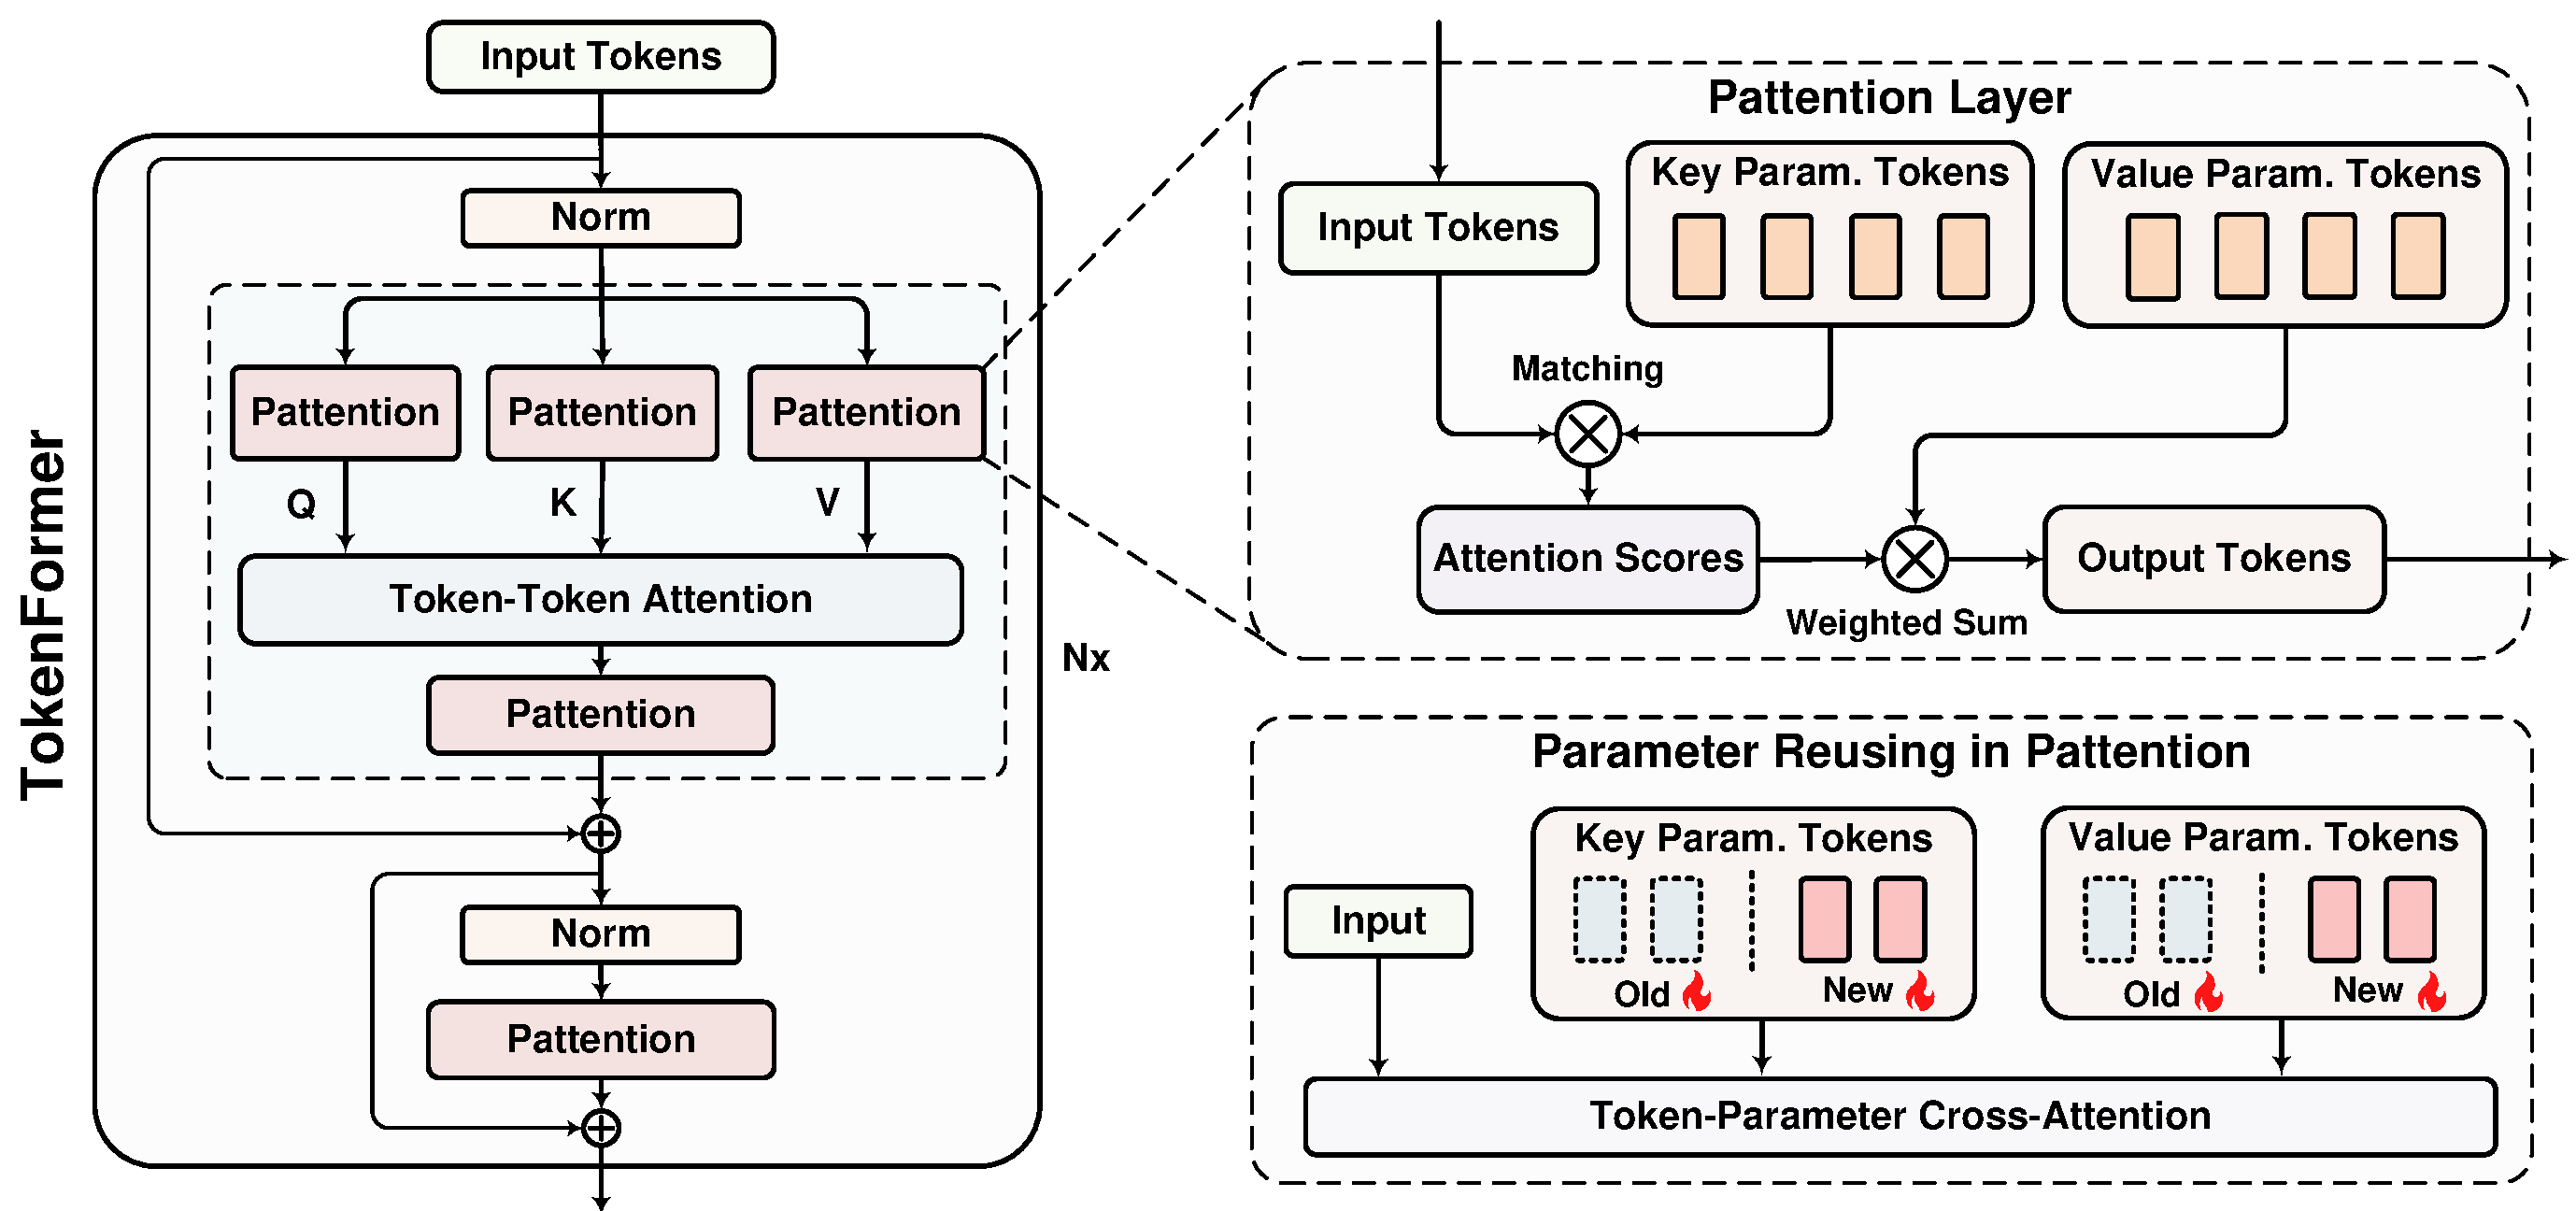
\includegraphics[width=0.99\linewidth]{./transformer-paper/arch2.pdf}
    \vspace{-0.1cm}
    \label{fig:tokenformer_figure}
    \vspace{-6pt}
\end{figure}
\end{frame}

\begin{frame}
\frametitle{Pattention Layer}
Let $K_P\in \mathbb{R}^{n\times d_1}$ and $V_P\in \mathbb{R}^{n\times d_2}$
represent the learnable parameter tokens.($n$ is the number of key-value pairs)
\begin{equation}
    \text{Pattention}(X,K_P,V_P)=\theta(X\cdot K_P^T)\cdot V_P,
\end{equation}
where $\theta$ is the modified softmax function. The output Pattention
scores, $S\in \mathbb{R}^{n\times n}$, are computed as:
\begin{equation}
    S_{ij} = \text{GeLU}\left(\frac{A_{ij} \times \tau}{\sqrt{\sum_{k=1}^n |A_{ik}|^2}}\right),
    ~~\forall~i,j \in 1...n,
\end{equation}
where $A=X\cdot K_P^T$ and $\tau$ is a scale factor.\\ \vspace{5pt}
In transformer, we have $Q=X\cdot W_Q$.\\
In tokenformer, we have $Q=\text{Pattention}(X,K_P^Q,V_P^Q)$.
\end{frame}

\begin{frame}
\frametitle{Overall Architecture}
\begin{itemize}
    \item QKV Pattention:$$Q=\text{Pattention}(X,K_P^Q,V_P^Q),~~
    K = \text{Pattention}(X,K_P^K,V_P^K),~~ V = \text{Pattention}(X,K_P^V,V_P^V).$$
    \item Token-Token Attention:
    $$X_{\text{att}}=\text{softmax}\left(\frac{Q\cdot K^T}{\sqrt{d}}\right)\cdot V,$$
    $$O_{\text{att}}=\text{Pattention}(X_{\text{att}},K_P^O,V_P^O).$$
    \item FFN:
    $$O_{\text{ffn}}=\text{Pattention}(O_{\text{att}},K_P^{\text{ffn}},V_P^{\text{ffn}}).$$
\end{itemize}
\end{frame}

\begin{frame}
\frametitle{Progressive Model Scaling}
Consider an existing Tokenformer model equipped with a
set of pre-trained key-value parameter tokens,
denoted as $K_P^{\text{old}}, V_P^{\text{old}} \in \mathbb{R}^{n \times d}$.
To scale the model, just augment this set by appending new key-value parameter
tokens $K_P^{\text{new}}, V_P^{\text{new}} \in \mathbb{R}^{m \times d}$ as
\begin{equation}
    K_P^{\text{scale}} = \left[K_P^{\text{old}}, K_P^{\text{new}}\right],
    ~~~~~V_P^{\text{scale}} = \left[V_P^{\text{old}}, V_P^{\text{new}}\right].
\end{equation}
\begin{equation}
    O = \text{Pattention}\left(X, K_P^{\text{scale}}, V_P^{\text{scale}}\right).
    \label{eq:token-parameter-3}
\end{equation}
Importantly, by initializing $K^{\text{new}}_P$ with zero,
the model can perfectly resume the model state from the pre-training
phase without losing the well-learned knowledge,
facilitating faster convergence and accelerating the overall scaling process.

\end{frame}